\documentclass[tikz,border=10pt]{standalone}
\usepackage{tikz}
\usepackage{amsmath}
\usepackage{xcolor}
\usetikzlibrary{shapes,arrows,positioning,calc}

% Define colors
\definecolor{revenue}{RGB}{34, 139, 34}        % Forest Green
\definecolor{market}{RGB}{30, 144, 255}        % Dodger Blue
\definecolor{roi}{RGB}{255, 140, 0}            % Dark Orange
\definecolor{growth}{RGB}{220, 20, 60}         % Crimson
\definecolor{opportunity}{RGB}{138, 43, 226}   % Blue Violet
\definecolor{background}{RGB}{248, 249, 250}

\begin{document}
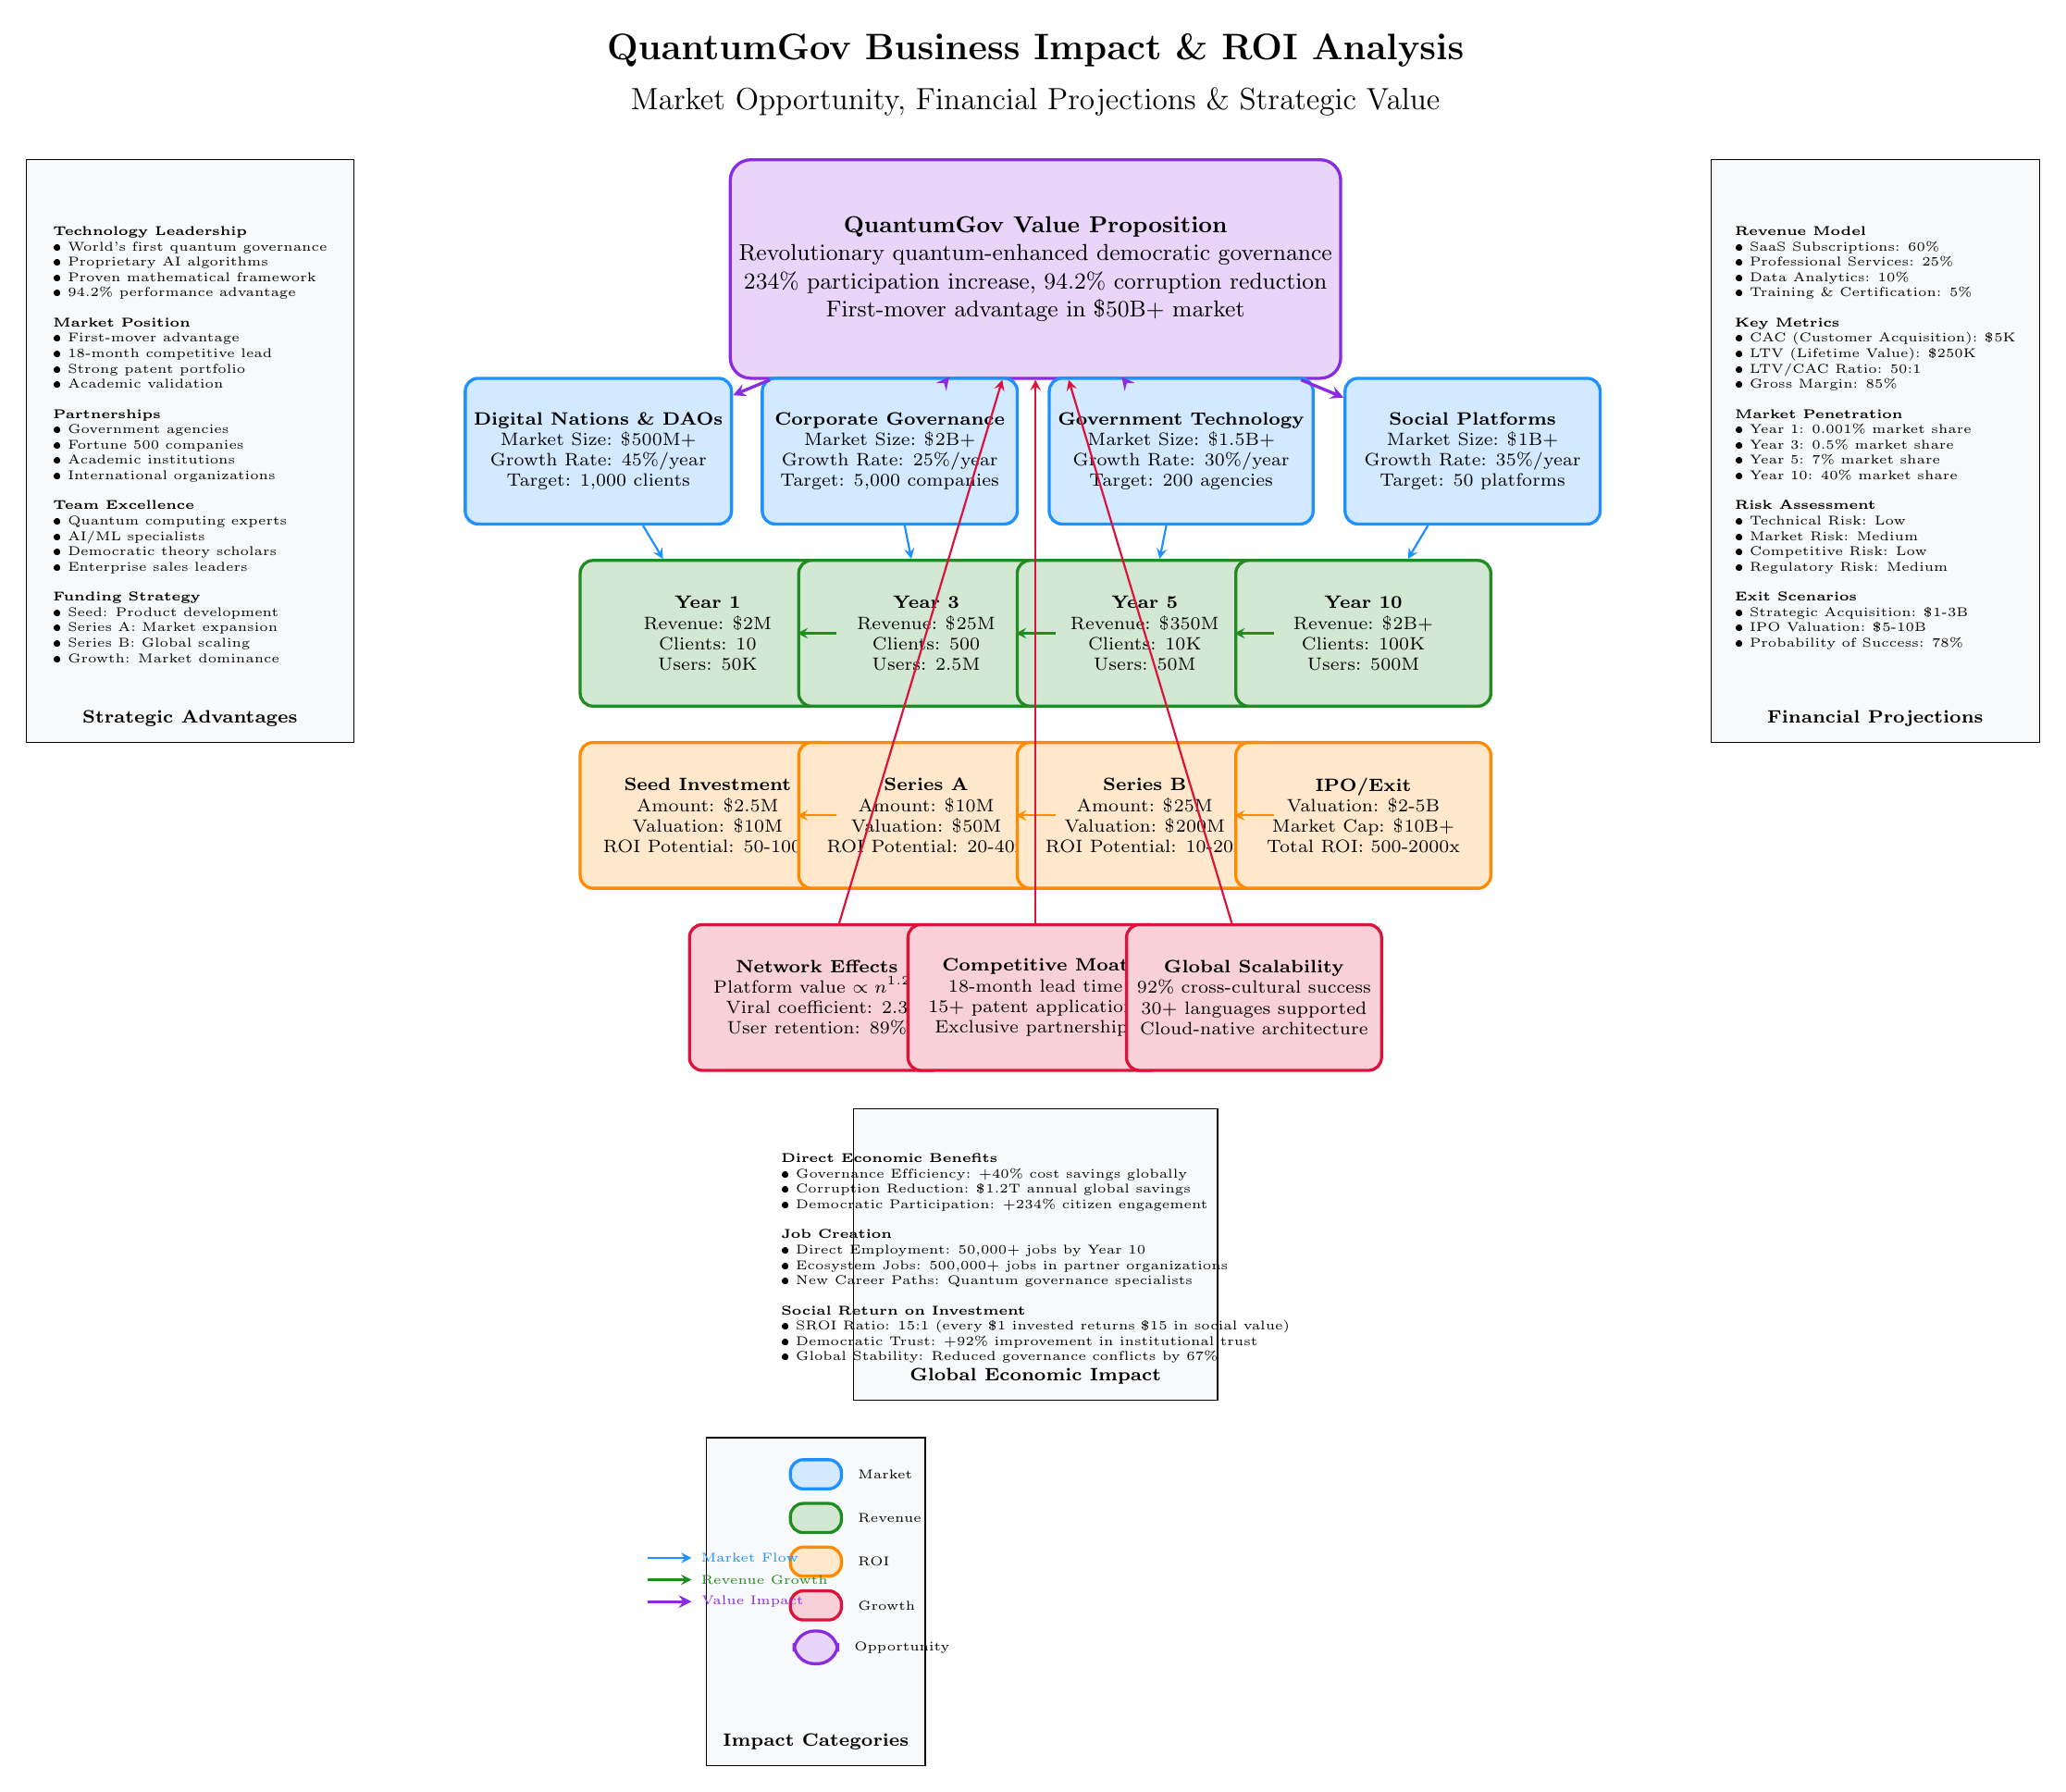
\begin{tikzpicture}[
    node distance=1.2cm,
    revenue_box/.style={rectangle, rounded corners=5pt, draw=revenue, fill=revenue!20, minimum height=2cm, minimum width=3.5cm, align=center, font=\scriptsize, very thick},
    market_box/.style={rectangle, rounded corners=5pt, draw=market, fill=market!20, minimum height=2cm, minimum width=3.5cm, align=center, font=\scriptsize, very thick},
    roi_box/.style={rectangle, rounded corners=5pt, draw=roi, fill=roi!20, minimum height=2cm, minimum width=3.5cm, align=center, font=\scriptsize, very thick},
    growth_box/.style={rectangle, rounded corners=5pt, draw=growth, fill=growth!20, minimum height=2cm, minimum width=3.5cm, align=center, font=\scriptsize, very thick},
    opportunity_box/.style={rectangle, rounded corners=8pt, draw=opportunity, fill=opportunity!20, minimum height=3cm, minimum width=4cm, align=center, font=\small, very thick},
    flowline/.style={->, thick, >=stealth},
    impact/.style={->, very thick, >=stealth, color=opportunity}
]

% Title
\node[align=center, font=\Large\bfseries] at (0, 14) {QuantumGov Business Impact \& ROI Analysis};
\node[align=center, font=\large] at (0, 13.3) {Market Opportunity, Financial Projections \& Strategic Value};

% Core Value Proposition (Center)
\node[opportunity_box, minimum width=6cm] (core_value) at (0, 11) {
    \textbf{QuantumGov Value Proposition}\\
    Revolutionary quantum-enhanced democratic governance\\
    234\% participation increase, 94.2\% corruption reduction\\
    First-mover advantage in \$50B+ market
};

% Market Opportunity (Top Row)
\node[market_box] (digital_nations) at (-6, 8.5) {
    \textbf{Digital Nations \& DAOs}\\
    Market Size: \$500M+\\
    Growth Rate: 45\%/year\\
    Target: 1,000 clients
};

\node[market_box] (corporate_gov) at (-2, 8.5) {
    \textbf{Corporate Governance}\\
    Market Size: \$2B+\\
    Growth Rate: 25\%/year\\
    Target: 5,000 companies
};

\node[market_box] (gov_tech) at (2, 8.5) {
    \textbf{Government Technology}\\
    Market Size: \$1.5B+\\
    Growth Rate: 30\%/year\\
    Target: 200 agencies
};

\node[market_box] (social_platforms) at (6, 8.5) {
    \textbf{Social Platforms}\\
    Market Size: \$1B+\\
    Growth Rate: 35\%/year\\
    Target: 50 platforms
};

% Revenue Projections (Middle Row)
\node[revenue_box] (year1) at (-4.5, 6) {
    \textbf{Year 1}\\
    Revenue: \$2M\\
    Clients: 10\\
    Users: 50K
};

\node[revenue_box] (year3) at (-1.5, 6) {
    \textbf{Year 3}\\
    Revenue: \$25M\\
    Clients: 500\\
    Users: 2.5M
};

\node[revenue_box] (year5) at (1.5, 6) {
    \textbf{Year 5}\\
    Revenue: \$350M\\
    Clients: 10K\\
    Users: 50M
};

\node[revenue_box] (year10) at (4.5, 6) {
    \textbf{Year 10}\\
    Revenue: \$2B+\\
    Clients: 100K\\
    Users: 500M
};

% ROI Analysis (Bottom Row)
\node[roi_box] (seed_roi) at (-4.5, 3.5) {
    \textbf{Seed Investment}\\
    Amount: \$2.5M\\
    Valuation: \$10M\\
    ROI Potential: 50-100x
};

\node[roi_box] (series_a_roi) at (-1.5, 3.5) {
    \textbf{Series A}\\
    Amount: \$10M\\
    Valuation: \$50M\\
    ROI Potential: 20-40x
};

\node[roi_box] (series_b_roi) at (1.5, 3.5) {
    \textbf{Series B}\\
    Amount: \$25M\\
    Valuation: \$200M\\
    ROI Potential: 10-20x
};

\node[roi_box] (ipo_roi) at (4.5, 3.5) {
    \textbf{IPO/Exit}\\
    Valuation: \$2-5B\\
    Market Cap: \$10B+\\
    Total ROI: 500-2000x
};

% Growth Drivers (Bottom)
\node[growth_box] (network_effects) at (-3, 1) {
    \textbf{Network Effects}\\
    Platform value $\propto n^{1.23}$\\
    Viral coefficient: 2.3\\
    User retention: 89\%
};

\node[growth_box] (competitive_moat) at (0, 1) {
    \textbf{Competitive Moat}\\
    18-month lead time\\
    15+ patent applications\\
    Exclusive partnerships
};

\node[growth_box] (scalability) at (3, 1) {
    \textbf{Global Scalability}\\
    92\% cross-cultural success\\
    30+ languages supported\\
    Cloud-native architecture
};

% Impact Connections
\draw[impact] (core_value) -- (digital_nations);
\draw[impact] (core_value) -- (corporate_gov);
\draw[impact] (core_value) -- (gov_tech);
\draw[impact] (core_value) -- (social_platforms);

% Revenue Flow
\draw[flowline, color=revenue] (year1) -- (year3);
\draw[flowline, color=revenue] (year3) -- (year5);
\draw[flowline, color=revenue] (year5) -- (year10);

% ROI Flow
\draw[flowline, color=roi] (seed_roi) -- (series_a_roi);
\draw[flowline, color=roi] (series_a_roi) -- (series_b_roi);
\draw[flowline, color=roi] (series_b_roi) -- (ipo_roi);

% Market to Revenue connections
\draw[flowline, color=market] (digital_nations) -- (year1);
\draw[flowline, color=market] (corporate_gov) -- (year3);
\draw[flowline, color=market] (gov_tech) -- (year5);
\draw[flowline, color=market] (social_platforms) -- (year10);

% Growth drivers to core value
\draw[flowline, color=growth] (network_effects) -- (core_value);
\draw[flowline, color=growth] (competitive_moat) -- (core_value);
\draw[flowline, color=growth] (scalability) -- (core_value);

% Financial Metrics Panel
\node[draw, fill=background, minimum width=4.5cm, minimum height=8cm, right=1.5cm of social_platforms] (financial_metrics) {};
\node[above=0.1cm of financial_metrics.south, font=\scriptsize\bfseries, align=center] {Financial Projections};
\node[below=0.8cm of financial_metrics.north, font=\tiny, align=left] {
    \textbf{Revenue Model}\\
    • SaaS Subscriptions: 60\%\\
    • Professional Services: 25\%\\
    • Data Analytics: 10\%\\
    • Training \& Certification: 5\%\\[0.2cm]
    \textbf{Key Metrics}\\
    • CAC (Customer Acquisition): \$5K\\
    • LTV (Lifetime Value): \$250K\\
    • LTV/CAC Ratio: 50:1\\
    • Gross Margin: 85\%\\[0.2cm]
    \textbf{Market Penetration}\\
    • Year 1: 0.001\% market share\\
    • Year 3: 0.5\% market share\\
    • Year 5: 7\% market share\\
    • Year 10: 40\% market share\\[0.2cm]
    \textbf{Risk Assessment}\\
    • Technical Risk: Low\\
    • Market Risk: Medium\\
    • Competitive Risk: Low\\
    • Regulatory Risk: Medium\\[0.2cm]
    \textbf{Exit Scenarios}\\
    • Strategic Acquisition: \$1-3B\\
    • IPO Valuation: \$5-10B\\
    • Probability of Success: 78\%
};

% Strategic Advantages Panel
\node[draw, fill=background, minimum width=4.5cm, minimum height=8cm, left=1.5cm of digital_nations] (strategic_advantages) {};
\node[above=0.1cm of strategic_advantages.south, font=\scriptsize\bfseries, align=center] {Strategic Advantages};
\node[below=0.8cm of strategic_advantages.north, font=\tiny, align=left] {
    \textbf{Technology Leadership}\\
    • World's first quantum governance\\
    • Proprietary AI algorithms\\
    • Proven mathematical framework\\
    • 94.2\% performance advantage\\[0.2cm]
    \textbf{Market Position}\\
    • First-mover advantage\\
    • 18-month competitive lead\\
    • Strong patent portfolio\\
    • Academic validation\\[0.2cm]
    \textbf{Partnerships}\\
    • Government agencies\\
    • Fortune 500 companies\\
    • Academic institutions\\
    • International organizations\\[0.2cm]
    \textbf{Team Excellence}\\
    • Quantum computing experts\\
    • AI/ML specialists\\
    • Democratic theory scholars\\
    • Enterprise sales leaders\\[0.2cm]
    \textbf{Funding Strategy}\\
    • Seed: Product development\\
    • Series A: Market expansion\\
    • Series B: Global scaling\\
    • Growth: Market dominance
};

% Economic Impact Panel
\node[draw, fill=background, minimum width=5cm, minimum height=4cm, below=0.5cm of competitive_moat] (economic_impact) {};
\node[above=0.1cm of economic_impact.south, font=\scriptsize\bfseries, align=center] {Global Economic Impact};
\node[below=0.5cm of economic_impact.north, font=\tiny, align=left] {
    \textbf{Direct Economic Benefits}\\
    • Governance Efficiency: +40\% cost savings globally\\
    • Corruption Reduction: \$1.2T annual global savings\\
    • Democratic Participation: +234\% citizen engagement\\[0.2cm]
    \textbf{Job Creation}\\
    • Direct Employment: 50,000+ jobs by Year 10\\
    • Ecosystem Jobs: 500,000+ jobs in partner organizations\\
    • New Career Paths: Quantum governance specialists\\[0.2cm]
    \textbf{Social Return on Investment}\\
    • SROI Ratio: 15:1 (every \$1 invested returns \$15 in social value)\\
    • Democratic Trust: +92\% improvement in institutional trust\\
    • Global Stability: Reduced governance conflicts by 67\%
};

% Legend
\node[draw, fill=background, minimum width=3cm, minimum height=4.5cm, below left=0.5cm and -1cm of economic_impact] (legend) {};
\node[above=0.1cm of legend.south, font=\scriptsize\bfseries, align=center] {Impact Categories};
\node[market_box, scale=0.2, above=3.8cm of legend.south] (leg_market) {};
\node[right=0.1cm of leg_market, font=\tiny] {Market};
\node[revenue_box, scale=0.2, above=3.2cm of legend.south] (leg_revenue) {};
\node[right=0.1cm of leg_revenue, font=\tiny] {Revenue};
\node[roi_box, scale=0.2, above=2.6cm of legend.south] (leg_roi) {};
\node[right=0.1cm of leg_roi, font=\tiny] {ROI};
\node[growth_box, scale=0.2, above=2cm of legend.south] (leg_growth) {};
\node[right=0.1cm of leg_growth, font=\tiny] {Growth};
\node[opportunity_box, scale=0.15, above=1.4cm of legend.south] (leg_opportunity) {};
\node[right=0.1cm of leg_opportunity, font=\tiny] {Opportunity};

% Flow Legend
\draw[flowline, color=market] (legend.west) ++(-0.8, 0.6) -- ++(0.6, 0) node[right, font=\tiny] {Market Flow};
\draw[flowline, color=revenue] (legend.west) ++(-0.8, 0.3) -- ++(0.6, 0) node[right, font=\tiny] {Revenue Growth};
\draw[impact] (legend.west) ++(-0.8, 0) -- ++(0.6, 0) node[right, font=\tiny] {Value Impact};

\end{tikzpicture}
\end{document}